\documentclass[a6paper,12pt]{article}
%\usepackage[T1]{fontenc}
\usepackage[british]{babel}
\usepackage[utf8]{inputenc}
\usepackage{float, graphicx,amsmath,amsfonts,cite,enumerate,tabularx}
\usepackage[final]{pdfpages}
\usepackage[margin=0.3in]{geometry}
\newcommand{\mel}[1]{\small\textbf{\textit{mel. #1 \\}}}


\setlength{\oddsidemargin}{-0.37in}
\setlength{\textwidth}{225pt}

\pagestyle{empty}

\begin{document}
\noindent Bortsupen av: .............................................
\vspace{50pt}
\begin{figure}[!h]
\centering

\includegraphics[width=\textwidth]{sangbok.png}
\end{figure}
\vspace{-20pt}
\begin{center}
\Huge\textbf{Kongl. Fysiks sångbok} \\
\Large anno 2019
\end{center}

\newpage
\setlength{\oddsidemargin}{-0.57in}
\noindent
\Large Vördade Fysiker... 

\footnotesize \noindent ...eller annan sångglad person! Du har nu nöjet att hålla i din hand 2019 års upplaga av Kongl. Fysiks sångbok!

Mellan dessa orangea pärmar finns de allra flesta sånger som sjungs på Fysiksektionen på KTH. Häri hittar du visor som passar såväl på gasque i Konsulatet, banquette på någon fin lokal eller varför inte bara hemma i glada vänners lag? Sångboken innehåller allt ifrån visor till sälla drycker till nidvisor till skojiga visor till vackra sånger, allt behändigt sorterat efter lämpligt (eller olämpligt) döpta kapitel. 

Vissa av låtarna har sjungits på KTH (eller andra lärosäten) i årtionden, och har ibland fått sig en liten uppdatering för att passa bättre med nutidens och sektionens värderingar. Andra är mer nyskrivna, och precis som förra året har vi valt att samla det bästa som skrevs och sjöngs under det gångna året på Teknisk Fysik i ett helt nytt kapitel som du finner längst bak i boken. Sångkulturen är i allra högsta grad levande på Fysik, och vi vill att sångboken ska utnyttja sin modulära natur för att spegla detta. 

Tack till alla som bidragit i år och alla som tidigare arbetat med sångboken, ingen nämnd och ingen glömd! Att få förvalta denna musikskatt är en ynnest och ett mycket hedersamt uppdrag som vi utför med glädje.

Mycket sångglädje önskas, och kom ihåg att starkt är vackert! 
\begin{flushright}
\textit{Adam Erlandsson och Filip af Malmborg, Förarlös\\ Sångboksansvariga 2019}
\end{flushright}


\newpage
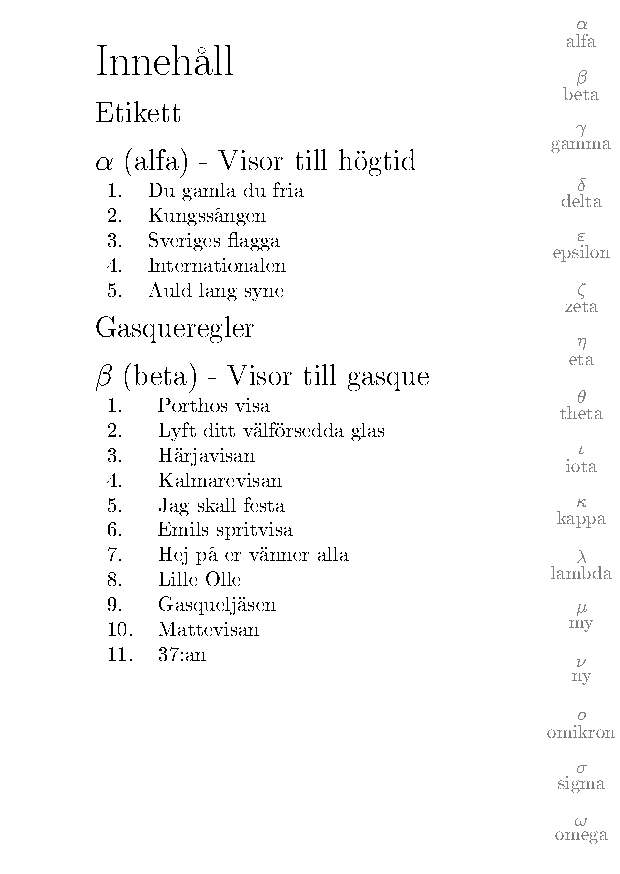
\includepdf[pages=1-6]{innehall.pdf}
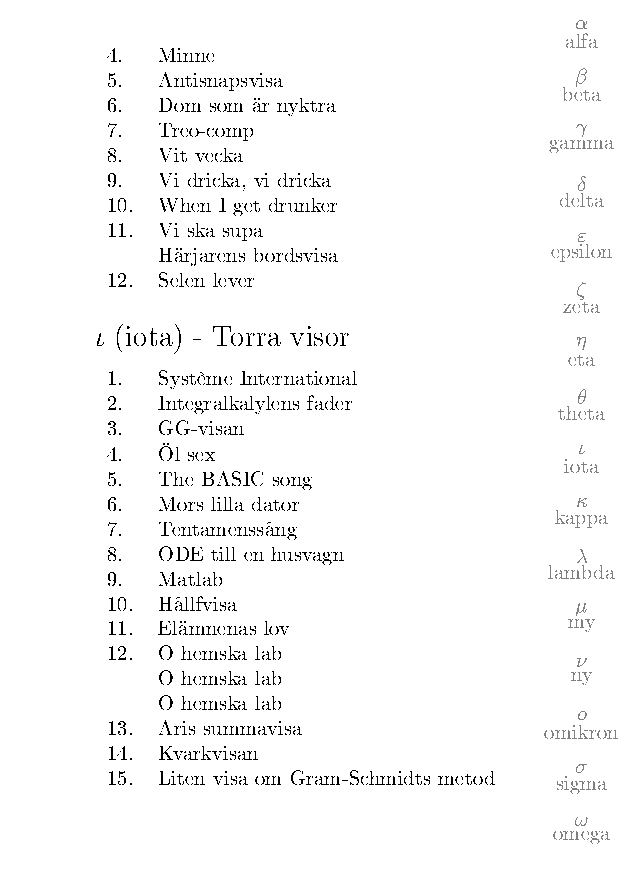
\includepdf[pages=1-5]{innehall2.pdf}

\newpage
\setlength{\oddsidemargin}{-0.57in}
\noindent
\Large Vettiquette\\
\footnotesize Vett- och etikettvärlden kan vid en första anblick verka snårig med otaliga regler som dessutom inte är skrivna i sten och därför är olika lite överallt. Men lugn - du kommer långt p vanlig hyfs och, ja, vett och det viktigaste tas upp här. Ettiquetten har långa anor och delar av den är förlegad, varför den alltid är i långsam förändring. Här presenterar jag en version där alla ska kunna känna sig inkluderade, som inte begränsar klädkoden utifrån kön och som inte förutsätter att ett visst kön behöver hjälp av ett annat utan som går bortom könen. Men mycket har levt kvar då det förhöjer stämningen och skapar en högtidlig atmosfär. Kanske är de regler du läser här lite annorlunda än vad du sett tidigare, men jag har här försökt utgå från hur Fysiksektionen och dess banquetter ser ut.\\
\normalsize\textbf{Klädkod}\\
\footnotesize På banquette är det klädkod högtidsdräkt som gäller. Det innebär vanligen balklänning eller frack men även militär högtidsuniform och högtidlig folkdräkt går bra. Vad gäller frack är det inga konstigheter - en frack är en frack. Balklänning är dock ett bredare begrepp men gemensamt för alla balklänningar är att de är golvlånga. Resten, så som mönster, färg och utformad spelar ingen större roll, så länge det är en festfin klänning. Även tvådelat går bra, så länge kjolen är golvlång.\\
Det finns även en mängd tillbehör som kan bäras vid en banquette, så som schmeck, handskar, medaljer, och sidenband. Vad gäller handskar bärs den korta 
\newpage
\setlength{\oddsidemargin}{-0.37in}
\noindent
varianten till frack och till klänning är det endast kutymt med handskar (och då är det den långa varianten som gäller) om klänningen har korta ärmar eller inga alls. Handsken ska ej kombineras med ringar utanpå, men en elegant klocka eller ett dito armband går bra. Under måltiden tas handskarna av men kan annars behållas på.\\
Schmecken är en studentikos mössa som lämpar sig vid högtidliga tillfällen. Till schmecken hör de färg-\\
glada spegaterna. Som fysiker sätter en på en orange spegat för varje påbörjat år och för varje frånvaroår en svart spegat. Schmecken kan bäras under hela banquetten. Vad gäller andra huvudbonader så ska hatt ej kombineras med frackklänning men hatt till frack är okej, och då är det cylindervarianten som gäller (även om detta är mycket ovanligt). Huvudpr-\\
ydnader som exempelvis diadem och fjädrar är vanligare och kan behållas på under hela tillställningen.\\
\normalsize\textbf{Etikett}\\
\footnotesize Banquetten börjar ofta med mingel innan det är dags att gå till bords. Då får du tillfälle att ta reda på vem din bordspartner är, om du inte går tillsammans med någon det vill säga. När banquetten ska börja leder du och din bordspartner varandra till bordet. Har någon av er en otymplig klänning är det kutymt att hjälpa till genom att dra ut stolen för henom.\\
Vid bordet hör det till god ordning att en konverserar med sin bordspartner, speciellt i början. När det är dags att skåla så ska du alltid skåla med öppen barm
\newpage
\setlength{\oddsidemargin}{-0.57in}
\noindent
till din partner. Det vill säga har du din partner till vänster om dig skålar du med höger arm. Du skålar först med din bordspartner, sedan med personen på andra sidan om dig och sist med personen mitt emot. När alla har druckit går en sedan i motsatt ordning och avslutar alltså skålen med sin bordspartner. Efter middagen är det i sedvanlig ordning dags för dans! Då leder ni varandra till dansgolvet och dansar, enligt tradition, den första dansen (en dans är två låtar) med varandra.\\
\normalsize\textbf{Vett}\\
\footnotesize Som jag sa i början kommer du långt med vanligt vett och lite hyfs, det är till exempel trevligt att hälla upp vatten till sin bordpartner om denna fått slut, även om det inte är någon regel. Och som jag även sa är reglerna inte skrivna i sten, ej heller dessa på Fysiksektionen. Det hör inte till ovanligheterna att en ser en fysiker i kortare knälång klänning eller i mörk kostym vid en banquette, och ingen kollar snett p a dig om du gör det. Att lägga dyra pengar på en balklänning eller en frack är inte en självklarhet. Inte heller lär någon bli arg om du glömmer bort i vilken ordning du ska skåla eller om du har en fråga om etiquettereglerna. Om en person ändå skulle bli arg är det hen som har begått det största etiquettebrottet, inte du. Har du någon övrig fundering rekommenderar jag dig att vända dig till en äldre fysiker eller etiquettdrottningen Magdalena Ribbing.\\
\indent Och med det önskar jag dig en fabulös kväll!
\begin{flushright}
\textit{Anna Karlhede, F-14}
\end{flushright}
\end{document}
